%-------------------------------------------------------------------------------
% File: main.tex
%	COVID-19 Behind the Numbers project documentation.
%
%	Compile using:
%	    $ pdflatex main.tex
%	    $ biber main
%
% Author: Rambod Rahmani <rambodrahmani@autistici.org>
%	  Created on 07/01/2021
%-------------------------------------------------------------------------------
\documentclass[11pt,a4paper]{article}

\usepackage[a4paper, portrait, margin=1.1in]{geometry}
\usepackage[dvipsnames]{xcolor}
\usepackage[linktoc=none]{hyperref}
\hypersetup{
	colorlinks=true,
	linkcolor=blue,
	filecolor=magenta,      
	urlcolor=blue,
}
\usepackage{listings}
\usepackage{float}
\usepackage{graphicx}
\usepackage[justification=centering]{caption}
\usepackage{wrapfig}
\usepackage{amsmath}
\usepackage{bold-extra}
\definecolor{anti-flashwhite}{rgb}{0.95, 0.95, 0.96}

% bibliography references
\usepackage[backend=biber,style=numeric,sorting=none]{biblatex}
\addbibresource{main.bib}
\nocite{*}

\begin{document}

%-------------------------------------------------------------------------------
% Title
%-------------------------------------------------------------------------------
\begin{center}
	\huge{\bfseries{\scshape{COVID-19: Behind the Numbers}}}\\
	\vspace{1.0cm}
	\large{Data Mining and Machine Learning Project}\\
	\vspace{0.2cm}
	\large{Prof. Marcelloni Francesco}\\
	\vspace{0.2cm}
	\large{Prof. Ducange Pietro}\\
	\vspace{1.0cm}
	\large\textit{Rambod Rahmani}\\
	\vspace{0.2cm}
	\scriptsize{Master's Degree in Artificial Intelligence and
	Data Engineering}\\
	\vspace{1.0cm}
	\normalsize{\today}
\end{center}

%-------------------------------------------------------------------------------
% Table of contents
%-------------------------------------------------------------------------------
\tableofcontents

%-------------------------------------------------------------------------------
% Section: Introduction
%-------------------------------------------------------------------------------
\section{Introduction}
\textbf{Decemebr 31, 2019}: \textit{Wuhan Municipal Health Commission, China,
reported a cluster of cases of pneumonia in Wuhan, Hubei Province. A novel
coronavirus was eventually identified.}\\
\textbf{January 1, 2020}: \textit{World Health Organization (WHO) had set up the
Incident Management Support Team across the three levels of the organization:
headquarters, regional headquarters and country level, putting the organization
on an emergency footing for dealing with the outbreak.}\\
\textbf{January 5, 2020}: \textit{WHO published the first Disease Outbreak News
on the new virus. This was a flagship technical publication to the scientific
and public health community as well as global media.}\\
\textbf{January 12, 2020}: \textit{China publicly shared the genetic sequence of
COVID-19.}\\
\\
At the beginning of 2020, a new virus started spreading around in the capital of
Central China's Hubei province: the city we all came to know as Wuhan. As it
turned out, this was the start of a world-changing event with overwhelming
extent: Coronavirus Disease 2019 (COVID-19). After the first wave of the virus
has passed over the entire world, the aim of this work is to address the
following questions:
\begin{itemize}
	\item Which countries have been affected the most by COVID-19?
	\item Which governments have taken the right actions to stop the
		spreading of the virus?
	\item Is it possible to build personalized predictive models for
		symptomatic COVID-19 patients based on basic health preconditions?
\end{itemize}
In order to fully answer these questions, first of all a reliable and big enough
dataset was needed. Second, Data Mining and Machine Learning techniques were
applied in order to obtain statistically significant results that could help
address the proposed questions. In the following pages the described work and
the resulting Python software is presented. The software architecture is
presented in the very last section in order to focus primarily on the dataset
retrieval and preprocessing, and on the analysis techniques and results.

%-------------------------------------------------------------------------------
% Section: Dataset
%-------------------------------------------------------------------------------
\section{Dataset}

%-------------------------------------------------------------------------------
% Section: Analysis
%-------------------------------------------------------------------------------
\section{Analysis}
As said in the introductory section, the analysis was carried out using data
mining and machine learning techniques in order to answer the proposed
questions. Each of the following subsections is focused on one of them.
\subsection{Which countries have been affected the most by COVID-19?}
To answer the very first question, we need to understand what is hidden behind
the official numbers and charts of confirmed COVID-19 active cases and deaths.
We are so used to watching them and sometimes we think we might even understand
how the COVID-19 pandemic is evolving as days goes by. For example, it is very
common to consider the following:
\begin{figure}[H]
    \begin{center}
        \hspace*{-1.8cm}
        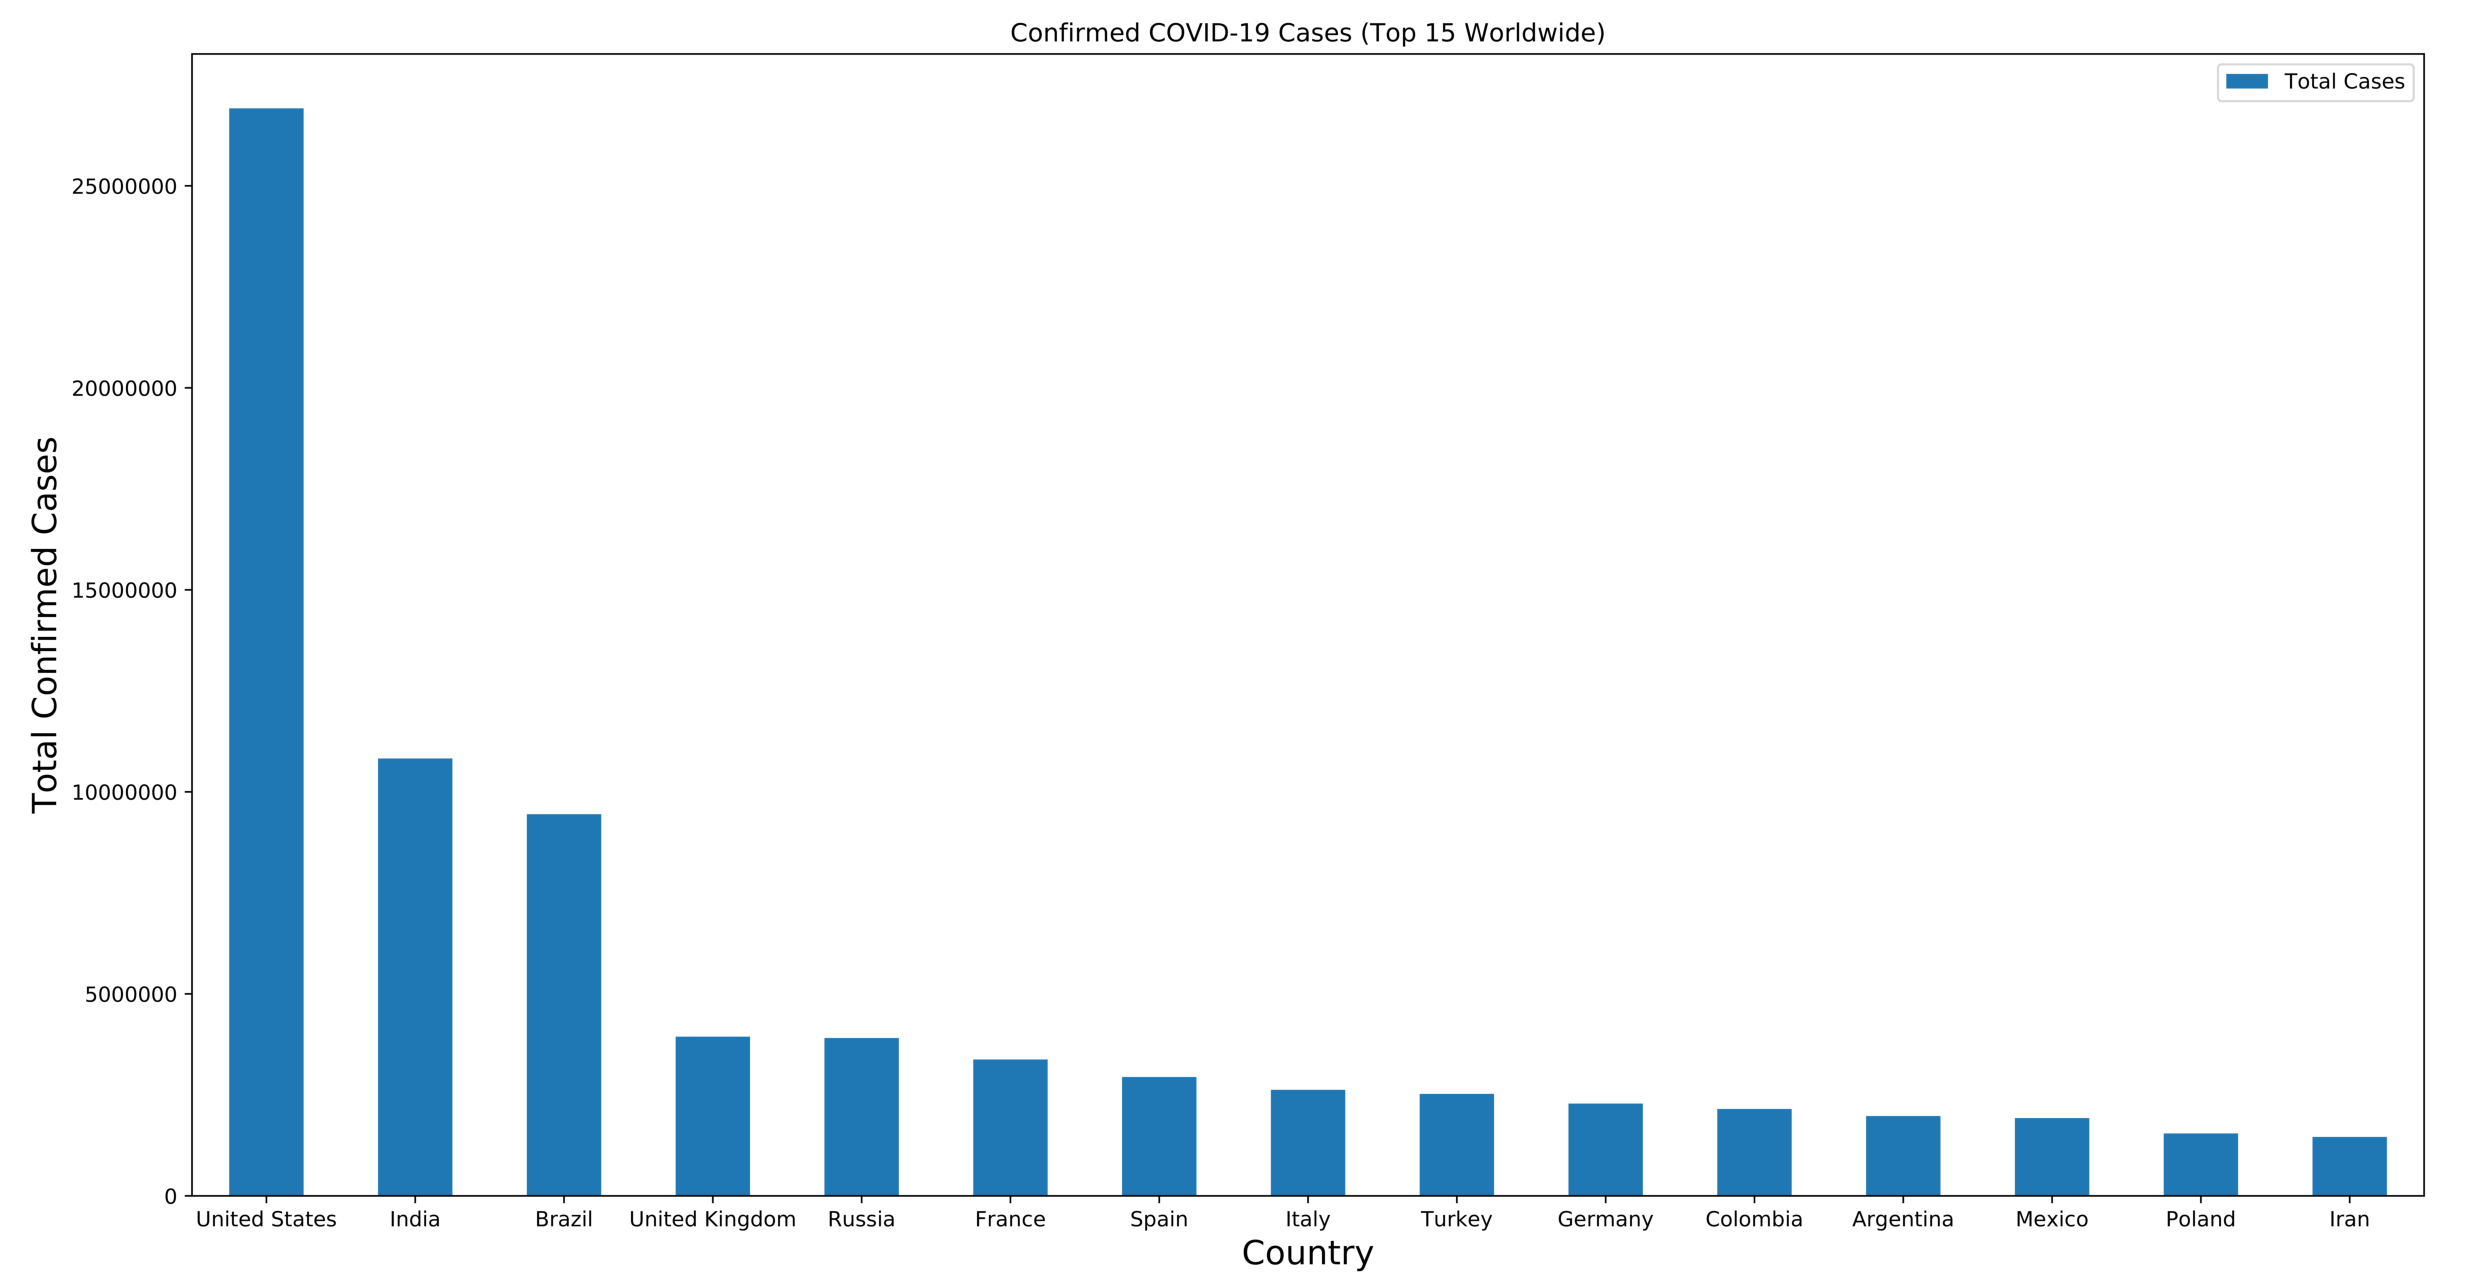
\includegraphics[scale=0.45]{img/top-15.pdf}
    \end{center}
    \vspace*{-0.4cm}
    \caption{Confirmed COVID-19 Cases Worldwide}
\end{figure}
\noindent Is this really the right choice? Does this ranking tells us anything
meaningful about the current undergoing pandemic situation? From what we can
observe in Figure 1, clearly United States has higher confirmed COVID-19 cases
than countries such as Spain or Italy. Taking into account that the US is a much
bigger country, we can agree that this results do not imply that the US is more
affected than Spain, Italy or Germany. We can therefore think of a fairer
comparison independent of the country size: the number of infections needs to be
normalized to the population of each country:
\begin{figure}[H]
    \begin{center}
        \hspace*{-1.7cm}
        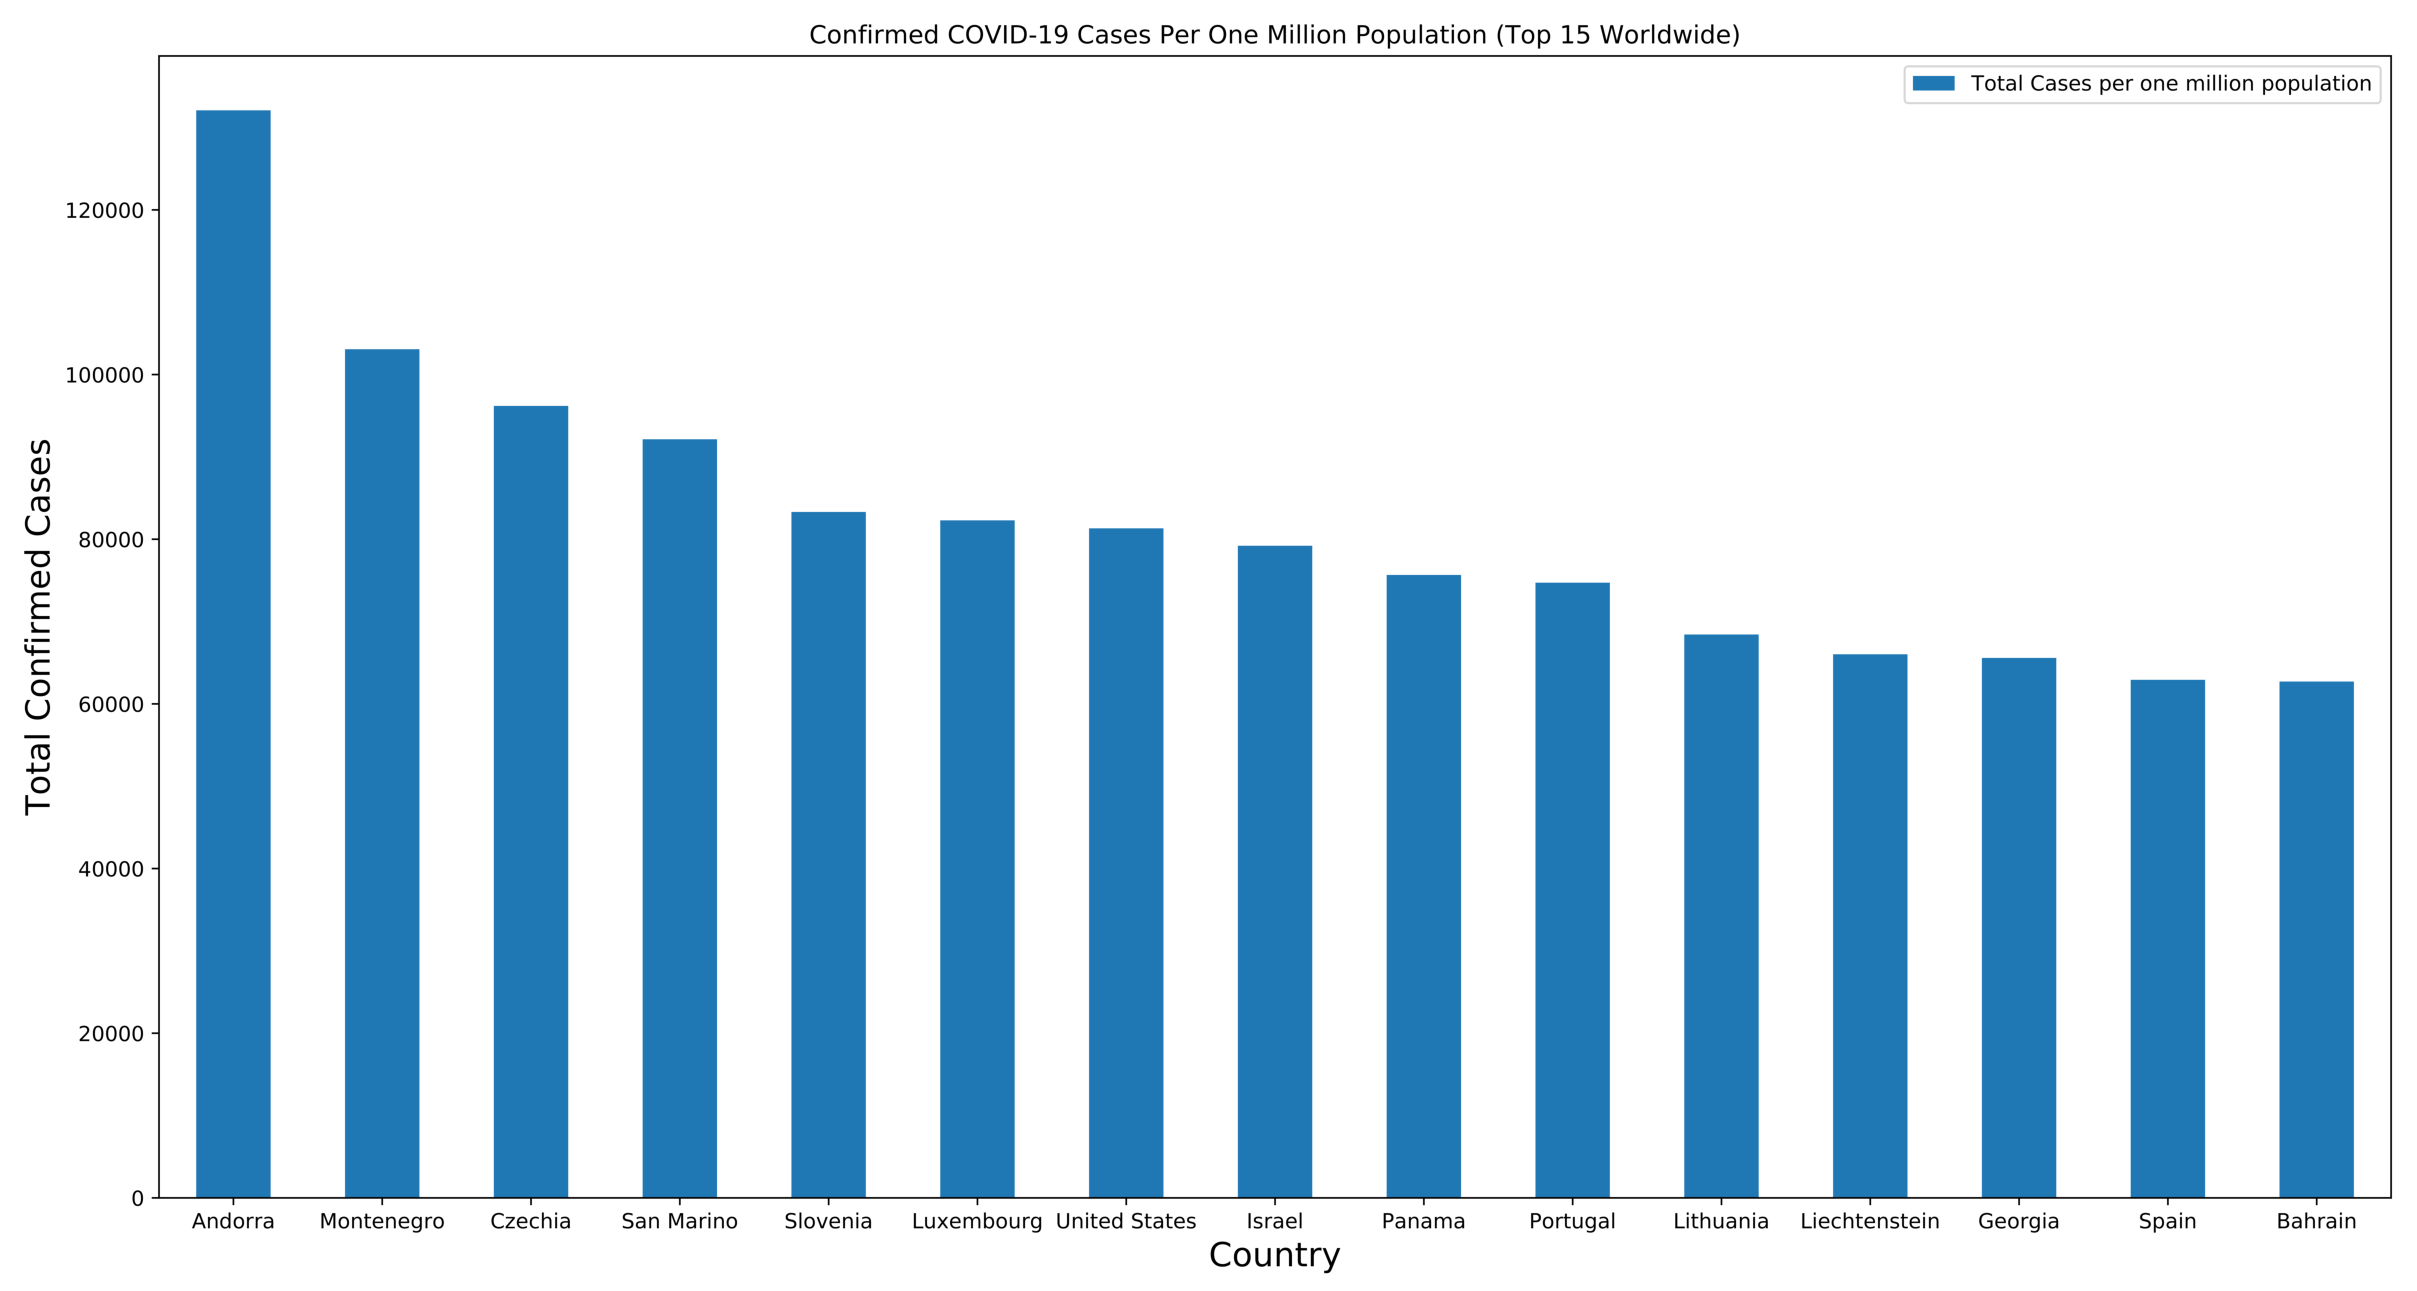
\includegraphics[scale=0.44]{img/top-15-per-million.pdf}
    \end{center}
    \vspace*{-0.4cm}
    \caption{Confirmed COVID-19 Cases Per One Million Population Worldwide}
\end{figure}
\noindent This provides a more coherent view of the countries most affected by
COVID-19, however it is not yet good enough: countries have different testing
policies and a more intensive COVID-19 testing rate gives more confirmed cases
while no testing at all would imply zero cases. We can all agree upon the fact
that zero cases with no testing at all does not really mean that a given country
is not affected by the pandemic. We therefore need a quantity unrelated to the
rate of testing.\\
This quantity is the number of deaths: this value is unbiased by the testing
rate. We will use the normalized number of deaths for comparing countries.
To summarize, by means of a machine learning algorithm applied to the COVID-19
data we organized countries into groups with similar epidemiological behavior.
Surprisingly, those groups form local clusters on the world map as well. This
unexpected insight helps us to answer the question proposed in this section.

\subsection{Which governments have taken the right actions?}
\subsection{Personalized predictive models for symptomatic COVID-19 patients}
		
%-------------------------------------------------------------------------------
% Section: Conclusion
%-------------------------------------------------------------------------------
\section{Conclusion}

%-------------------------------------------------------------------------------
% Section: Software Architecture
%-------------------------------------------------------------------------------
\section{Software Architecture}

\printbibliography

\end{document}
